\documentclass[12pt,a4paper]{article}
\usepackage[a4paper, total={6.95in, 9.7in}]{geometry}
\usepackage[utf8]{inputenc}
\usepackage{graphicx}
\usepackage{amsmath}
\usepackage{amssymb}
\usepackage{amsthm}
\usepackage{subfigure}
\usepackage{bm}

\setlength{\parindent}{0pt}


\author{\vspace{1mm}
  Paul Hill}

\date{\vspace{1mm} % Datumsfeld einrichten
       \today}

\thispagestyle{empty} % Die Titelseite soll keine Seitenzahl bekommen...[1]
%\end{titlepage}


\title{Neuro-Backprop}
\date{August 2020}

\begin{document}

\maketitle

\begin{figure*}[!ht]
  \centering
  \subfigure[random caption 1]{\includegraphics[height=0.35\linewidth]{img/pyramidial.png}}\quad
  \subfigure[random caption 2]{\includegraphics[height=0.35\linewidth]{img/pyr_abstract.png}}\quad
  \subfigure[random caption 1]{\includegraphics[height=0.35\linewidth]{img/inter.png}}\quad
  \subfigure[random caption 2]{\includegraphics[height=0.2\linewidth]{img/inter_abstract.png}}
\end{figure*}

\section{Introduction}
\subsection{Multicompartment-Neurons}
Real nerve-cells usually have a spatial extension much larger than their actual cell-bodies (somas). To model the spatial variation of electric potentials over such cells (specifically the cell's dendrites), which is due to the finite speed with which electric signals propagate, one introduces several distinct compartments that are coupled to each other. The potential of the soma-compartment is then given by
\begin{equation}
\dot{u} = -g_lu + \sum_xg_x(v_x-u) + I_{syn}, \label{eq:soma}
\end{equation}  
where $g_l$ is the leakage conductance of the soma, $x$ runs over all connected compartments of the cell and $g_x$ is the respective conductance coupling $x$ to the soma. $I_{syn}$ accounts for an additional current input coupled directly into the soma. In our case we will always have $I_{syn} = g_{som}(u_{ex}-u)$, where $u_{ex}$ is any external potential.\\
Note that \eqref{eq:soma} behaves as a low-pass filter for the potentials $u_x$ and $u_{ex}$ with time constant $\tau = \frac{1}{g_{tot}} = \frac{1}{g_l + \sum_x g_x + g_{som}}$. For imprinted signals with time scale $T\gg\tau$ the soma potentials takes on the form (steady-state solution)
\begin{equation}
\tilde{u} = \frac{1}{g_{tot}}\left(\sum_x g_xu_x + g_{som}u_{ex}\right).
\end{equation}

Furthermore we restrict our model to the rate-based case in which synaptic inputs are given in terms of the firing rates of their presynaptic partners $r_y$
\begin{equation}
v_x = \sum_yW_{xy}r_y = \sum_yW_{xy}\phi(u_y).
\end{equation}
Here the vector $\bm{W}_x$ denotes the coupling between the the presynaptic partners and the $x$-compartment and firing rates are given in terms of the corresponding soma potentials $u_y$ via the activation function $\phi(u_y)$.

\subsection{PyraL-Network }
The network approximating the backpropagation-algorithm is built upon two kind of neurons, pyrimidial- and lateral inter-neurons. The first one consists of two compartments beside the soma, the basal and apical dendrites. \eqref{eq:soma} takes on the form
\begin{equation}
\dot{u}^P = -g_lu^P + g_B(v^P_B - u^P) + g_A(v^P_A - u^P), 
\end{equation}
where $B$ denotes the basal and $A$ the apical compartment.
The inter-neurons on the other hand are governed by
\begin{equation}
\dot{u}^I = -g_lu^I + g_D(v^I_D - u^I) + g_{som}(u_{ex} - u^I),
\end{equation}
where $D$ denotes the dendritic compartment and we have an external potential $u_{ex}$ directly coupled into the soma. Fig. ???? depicts both neuron types in their biological manifestation and abstract description, respectively.

With these two types of neurons one is now able to go on and build larger networks as the one depicted in Fig. \ref{fig:network}.

\begin{figure*}[!ht]
  \centering
  \includegraphics[height=0.6\linewidth]{img/network.png}
  \label{fig:network}
\end{figure*}

The network dynamics for $N$ layers ($N-2$ hidden layers) are governed by the following set of equations (for $0<k<N$) 
\begin{align}
\dot{\bm{u}}^P_k &= -g_l\bm{u}^P_k + g_B(\bm{v}^P_{B,k} - \bm{u}^P_k) + g_A(\bm{v}^P_{A,k} - \bm{u}^P_k)\\
\dot{\bm{u}}^I_k &= -g_l\bm{u}^I_k + g_D(\bm{v}^I_{D,k} - \bm{u}^I_k) + g_{som}(\bm{u}^P_{k+1} - \bm{u}^I_k)\\
\bm{v}^P_{B,k} &= \bm{W}^{up}_k\phi(\bm{u}^P_{k-1})\\
\bm{v}^P_{A,k} &= \bm{W}^{pi}_k\phi(\bm{u}^I_{k}) + \bm{W}^{down}_k\phi(\bm{u}^P_{k+1})\\\label{eq:apical}
\bm{v}^I_{D,k} &= \bm{W}^{ip}_k\phi(\bm{u}^P_{k}),
\end{align}
where $\bm{W}$ are now matrices, $\bm{v},\bm{u}$ are vectors and $k$ is the layer index ($k=0$ is the input layer).\\
The output neurons look slightly different,
\begin{align}
\dot{\bm{u}}^P_N &= -g_l\bm{u}^P_N + g_B(\bm{v}^P_{B,N} - \bm{u}^P_N) + g_{som}(\bm{u}^{target} - \bm{u}^P_N)\\
\bm{v}^P_{B,N} &= \bm{W}^{up}_N\phi(\bm{u}^P_{N-1}).
\end{align}

Note that, provided the network reaches a (unique) fix-point, i.e. a configuration in which all derivatives of the soma potentials vanish simultaneously, the network essentially maps the input rates (or input potentials) of the $0$-th layer to the output rates obtained from the $N$-th layer. It is this non-linear mapping between input and output rates that eventually enables the network to solve complex classification and regression tasks by adjusting the strength of its synaptic connections $\bm{W}$. However, the existence (and uniqueness) of a fix-point of the underlaying network dynamics depends non-trivially on the weights $\bm{W}$ and conductances $g$. 

\subsection{Learning-rules}
Assuming the network indeed converges to a stable fix-point for the given input rates, there is yet no mechanism that makes the output potentials reproduce a given target signal $\bm{u}^{target}$. To solve this the concept of dendritic prediction of somatic spiking rates is introduced. Consider therefore a pyramidial neuron in the output layer when teaching is disabled ($g_{som}=0$). The soma potential is then, in steady-state, given by
\begin{equation}
\hat{\bm{v}}^P_{B,N} \equiv \tilde{\bm{u}}^P = \frac{g_B}{g_l + g_B}\bm{W}r^P_{N-1}.
\end{equation} 
When teaching is enabled, $\tilde{u}^P$ is nudged away from the dendritic prediction $\hat{v}^P$ towards
\begin{equation}
\tilde{\bm{u}}^P_N = (1-\lambda_{out})\hat{\bm{v}}^P_{B,N} + \lambda_{out}\bm{u}^{target},
\end{equation}
with $\lambda_{out} = \frac{g_{som}}{g_l + g_B + g_{som}}$.
The difference in predicted and actual firing rate $\phi(u^P) - \phi(\hat{v}^P)$ can now be used to update the synaptic strengths such that $\hat{v}^P$ is itself nudged towards $u^{target}$ and eventually $\tilde{u}^P = \hat{v}^p$ holds again.\\
Similar equations hold for hidden pyramidial neurons and inter-neurons as well
\begin{align}
\tilde{u}^P_k &= \hat{\bm{v}}^P_{B,k} + \lambda_{hid}\bm{v}^P_{A,k}, \quad \lambda_{hid} = \frac{g_A}{g_l + g_B + g_A}\\
\tilde{u}^I_k &= (1-\lambda_I)\hat{v}^I_{D,k} + \lambda_{I}u^P_{k+1}, \quad \lambda_{I} = \frac{g_{som}}{g_l + g_D + g_{som}},
\end{align}
with $\hat{\bm{v}}^P_{B,k} = \frac{g_B}{g_l + g_B + g_A}\bm{W}^{up}_kr^P_{k-1}$ and $\hat{\bm{v}}^I_{D,k} = \frac{g_D}{g_l + g_D}\bm{W}^{ip}_kr^P_k$.\\

Finally, updating of the weights is realized by first low-pass filtering the dendritic prediction error with time constant $\tau_w$
\begin{align}
\tau_w\dot{\bm{\Delta}}^{up}_k &= \left(\phi(\bm{u}^P_k - \phi(\hat{\bm{v}}^P_{B,k})\right)(r^P_{k-1})^T\\\label{eq:delta_up}
\tau_w\dot{\bm{\Delta}}^{ip}_k &= \left(\phi(\bm{u}^I_k - \phi(\hat{\bm{v}}^I_{D,k})\right)(r^P_{k})^T\\
\tau_w\dot{\bm{\Delta}}^{pi}_k &= -\bm{v}^P_A(r^I_{k})^T \label{eq:delta_ap}
\end{align}
and then integrating
\begin{align}
\frac{d\bm{W}^{up}_k}{dt} &= \eta^{up}_k\bm{\Delta}^{up}_k \\
\frac{d\bm{W}^{ip}_k}{dt} &= \eta^{ip}_k\bm{\Delta}^{ip}_k \\
\frac{d\bm{W}^{pi}_k}{dt} &= \eta^{pi}_k\bm{\Delta}^{pi}_k.
\end{align}
Note that, based on eq. \eqref{eq:delta_up} - \eqref{eq:delta_ap}, output neurons change to predict the target signal, inter-neurons change to predict the pyramidial neurons of the next layer, hidden pyramidial neurons are driven by their apical compartment and finally the apical compartment adjust the lateral $\bm{W}^{pi}$ weights such that the top-down (see eq. \eqref{eq:apical}) is canceled and the apical potential becomes zero.\\

\subsubsection{Self-predicting state}
Especially when no target signal is applied this mechanism drives the network in what is called the self-predicting state. It is characterized by the cancellation of all apical potentials and when inter-neuron soma potentials match the pyramidial soma potentials of the next layer, i.e.
\begin{align}
\bm{v}^P_A &= 0\\
\hat{\bm{v}}^I_{D,k} &= \hat{\bm{v}}^P_{B,k+1},
\end{align} 
which is equivalently expressed as 
\begin{align}
\bm{W}^{pi}_k &= - \bm{W}^{down}_k\\
\bm{W}^{ip}_k &= \frac{g_l + g_D}{g_l + g_B + g_A}\frac{g_B}{g_D}\bm{W}^{up}_{k+1},
\end{align}
with $g_A = 0$ for the output layer. Since in the self-predicting state all apical compartments vanish the network is garuanteed to have a fix-point and behaves like a artificial neural network with same forward weights ($\sim \bm{W}^{up}$) and activation function. 


\subsection{Approximation of the error-backpropagation algorithm}
Starting from the the self-predicting state we now switch on the teaching signal $\bm{u}^{target}$, where throughout small couplings $\lambda = \lambda_{out} = \lambda_I = \lambda_{hid}\ll 1$ are assumed.\\
Doing so nudges the output potential away from $\hat{\bm{v}}^P_{B,N} = \tilde{\bm{u}}^I_{N-1}$, resulting in a change of the apical potential in the previous layer as
\begin{equation}
\bm{v}^P_{N-1} = \bm{W}^{down}_{N-1}\underbrace{\left(\phi(\tilde{\bm{u}}^P_N) - \phi(\hat{\bm{v}}^P_{B, N})\right)}_{\bm{e}_N} \approx \lambda\bm{W}^{down}_{N-1}\phi'(\hat{\bm{v}}^P_{B, N})\left(\bm{u}^{target} - \hat{\bm{v}}^P_{N}\right)\equiv \lambda\bm{W}^{down}_{N-1}\bm{D}_N\left(\bm{u}^{target} - \hat{\bm{v}}^P_{N}\right),
\end{equation}
where the prediction error $\bm{e}_N$ was introduced. This error propagates further down the network
\begin{equation}
\bm{e}_{N-1} = \phi(\tilde{\bm{u}}^P_{N-1}) - \phi(\hat{\bm{v}}^P_{B,N-1}) \approx \phi'(\hat{\bm{v}}^P_{B,N-1}) \lambda \bm{W}^{down}_{N-1}\bm{e}_N = \lambda^2 \bm{D}_{N-1}\bm{W}^{down}_{N-1}\bm{D}_N\left(\bm{u}^{target} - \hat{\bm{v}}^P_{N}\right).
\end{equation}
\end{document}
